% -- Introduction ---------------------------------------
\section{Introduction}
For the lab, a computational intensive kernel has to be extracted from the x264 software application, which is a free software library for encoding video stream into H.236/MPEG-4 AVC format. It is able to use Periodic Intra Refresh instead of keyframes used by H.264, refreshing the image of the video by moving a column of intra blocks from one side of the screen to the other. This hides the refreshing effect from the user while the frame loads. The \mcode{x264} application is executed on a FPGA running a MicroBlaze host processor. By running the particular kernel on the $\rho$-VEX co-processor, the execution time can be decreased by making use of parallel processing. 

\section{Exploring the x264 application}
Duing the first lab we got familiar with the x264 application, a powerful coding tool to remove temporal redundancy by using motion estimation. In Section \ref{sec:intensive} we will discuss the various computational intenstive kernels within the x264 algorithm. The choosen kernel will be explained in Section \ref{sec:kernel}, the provided memory layout of the FPGA architecture in Section \ref{sec:layout} and the actual implementation will be discussed in Section \ref{sec:executing}.

\subsection{Detecting the Computationally Most Intensive Kernel}
\label{sec:intensive}
A few input files are provided in the first lab to demonstrate the compile and run commands of the x264 application. The \mcode{.y4m} input files are decoded to create a short \mcode{.mkv} movie using this command in the terminal: \mcode{.\/x264 eledream\_64x32\_3.y4m -o testframe.mkv}. By adding the \mcode{gprof} flag to the compile command, a list is created of all functions ordered by their share of the total execution time (in percentage). The number of function calls is also shown, as well as the total execution time for each input file. These five input \mcode{.y4m} files vary in resolution (either 64x32 or 640x320 pixels) and amount of frames (either 1, 3, 8, 32 or 128). Profiling the x264 execution for the \mcode{.y4m} files that are provided by the lab leads to the ranking show in table \ref{tab:chart}.

% -- GPROF uitslagen ---------------------------------------
\begin{table}[htb]%
\centering
\small
	\begin{tabular}{lclll}
		\centering
		\bf{Input file} & \bf{Time (sec)} 	& \bf{Share ($\%$)} & \bf{Calls}	& \bf{Kernel name} \\ \cline{1-5}
		\multirow{3}{*}{eledream\_32x18\_1.y4m}	&				& 100.00	& 71		&	x264\_analyse\_init\_costs\\ 
																						&	0.02	& 0.00 		& 1646	&	x264\_free\\ 
																						&				& 0.00		& 784		&	x264\_cabac\_encode\_desicion\_c\\ \cline{1-5}
		\multirow{3}{*}{eledream\_64x32\_3.y4m} & 			& 66.67		& 71		& x264\_analyse\_init\_costs\\
																						&	0.03	& 33.33 	& 1971	&	x264\_pixel\_satd\_4x4\\ 
																						&				& 0.00		& 4830	&	x264\_pixel\_satd\_8x4\\ \cline{1-5}
		\multirow{3}{*}{eledream\_640x320\_8.y4m}	& 			& 14.29	& 1599044		&	x264\_pixel\_satd\_8x4\\ 
																							&	1.61	& 11.80 	& 570708	&	x264\_get\_ref\\ 
																							&				& 4.97		& 38770		&	x264\_pixel\_satd\_x4\_16x16\\ \cline{1-5}
		\multirow{3}{*}{eledream\_640x320\_32.y4m}& 			& 20.61		& 7228633		&	get\_ref\\ 
																							& 8.54	& 13.23 	& 15386501	&	x264\_pixel\_satd\_8x4\\ 
																							&				& 4.57		& 1009690		&	x264\_pixel\_satd\_x4\_8x8\\ \cline{1-5}
		\multirow{3}{*}{eledream\_640x320\_128.y4m}&			& 17.48		& 21956292	&	get\_ref\\
																							&	 29.86& 14.17 	& 49862831	&	x264\_pixel\_satd\_8x4\\
																							&				& 6.56		& 1023315		&	x264\_pixel\_satd\_x4\_16x16\\ \cline{1-5}
	\end{tabular}	
\caption{Chart with computationally most intensive kernels for each input stream.}
\label{tab:chart}
\end{table}

\subsection{The \mcode{pixel_satd_8x4} kernel}
\label{sec:kernel}
Given these statistics, we decide to extract the \mcode{x264\_pixel\_satd\_8x4 kernel}, since it has a fair share in the execution time and was advised by the teaching assistants. This kernel evaluates the Sum of Transformed Differences (SATD) between a 8x4 pixel block from the input stream and reference blocks. The SATD is a metric used for video compression where the differences between the pixels are taken and put into a frequency transform, usually a Hadamard transform. These blocks can have various sizes depending on the inputs and constraint of the system varying from 4x4 pixel blocks to 8x4 blocks and even 16x16 blocks. The reference block with the lowest SATD value can be used to estimate motion in video coding to remove temporal redundancy. 

\subsection{Memory layout of the MicroBlaze}
\label{sec:layout}

When writing pixels to the $\rho$-VEX for SATD calculation, these pixels need to be picked from the MicroBlaze memory. However, these pixels are not written as one block of contiguous bytes. Rows of four bytes (MicroBlaze has 32-bit registers) are interrupted by a fixed amount of memory called a stride. This value is often given in bytes to be skipped in order to continue reading the particular data file. Figure \ref{fig:stride} shows the concept of strides for two pixels from the MicroBlaze memory, which are splitted into two rows of 4 bytes since a pixels consists of eight bytes. When writing data to the $\rho$-VEX memory we use a stride of four bytes, resulting in a configuration as shown in figure \ref{fig:testpixels}
% -- Plaatje Stride ------------------------------

\begin{figure}[htb]
	\centering
	\begin{subfigure}{0.3\textwidth}
		\centering
		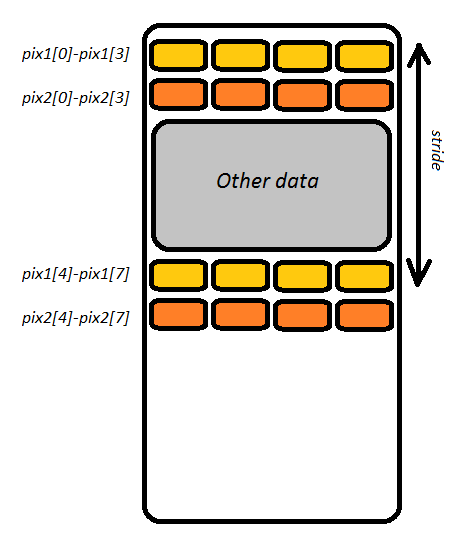
\includegraphics[width=150px]{Pictures/stride}
		\caption{Large stride in MicroBlaze memory}
		\label{fig:stride}
	\end{subfigure}
	\quad
	\begin{subfigure}{0.3\textwidth}
		\centering
		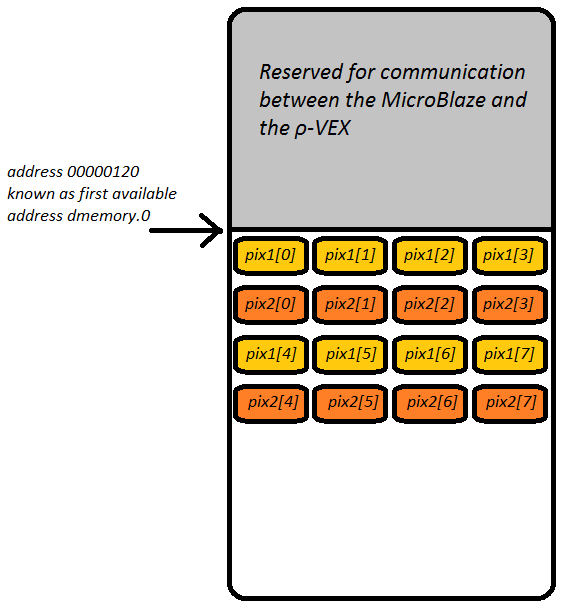
\includegraphics[width=150px]{Pictures/pixels_dmem}
		\caption{Four byte strid in $\rho$-VEX data memory}
		\label{fig:testpixels}
	\end{subfigure}
\caption{MicroBlaze memory uses strides to split up data files}%
\label{}%
\end{figure}

\subsection{Executing an Application on the Development Board and $\rho$-VEX}
\label{sec:executing}
When executing \mcode{./configure}, a file is created for configuration of the application. However, the resulting \mcode{config.mak} file is made for applications running on the guest (Ubuntu). In order to configure for MicroBlaze, the \mcode{config.mak} file has to altered. All references to \mcode{m32} have to be removed and the \mcode{--DWORDS\_BIGENDIAN} flag has to be added to the \mcode{CFLAGS} variable. This has to be done everytime when configurating the application for MicroBlaze.

After doing this, the application now can be 'made' for MicroBlaze by first moving to the Scratchbox 2 environment for MicroBlaze and then execute the \mcode{make} command. Figure \ref{fig:lelijk} shows a block diagram of both the platforms.

% -- Plaatje Practicum Evnvironments ------------------------------
\begin{figure}[htb]%
\centering
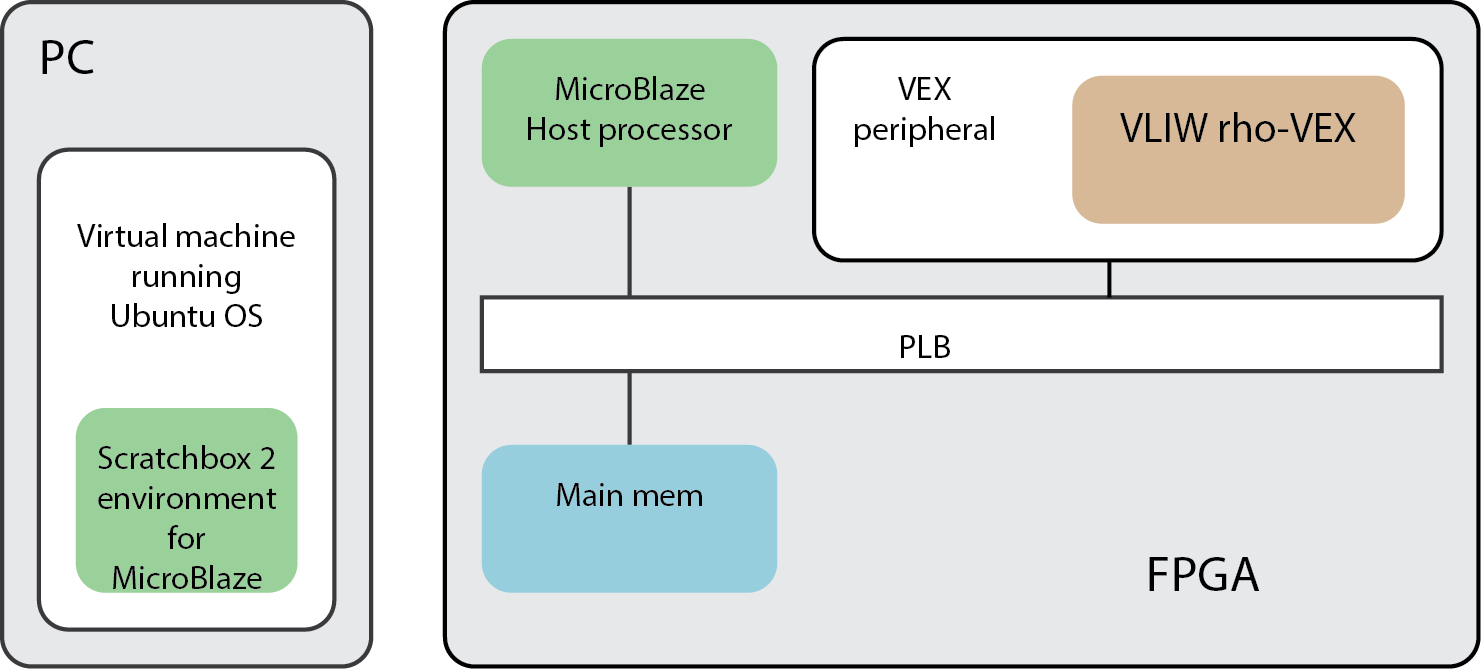
\includegraphics[width=300px]{Pictures/platform}%
\caption{Block diagram of the Virtual Machine and the ERA platform}%
\label{fig:lelijk}%
\end{figure}

In order to run the application on the MicroBlaze host processor, the \mcode{x264} executable must be compressed along with an input stream in a \mcode{tar.gz} file. This file can be put, via the MicroBlaze host processor, on one of the three FPGAs using the \mcode{scp}, \mcode{ftp} and \mcode{put} command. In order to connect the programmer to the development board, one must use the \mcode{ssh} and \mcode{telnet} command. See also figure \ref{fig:hoppen}.


% -- Plaatje Ubuntu-commando's ------------------------------
\begin{figure}[htb]%
\centering
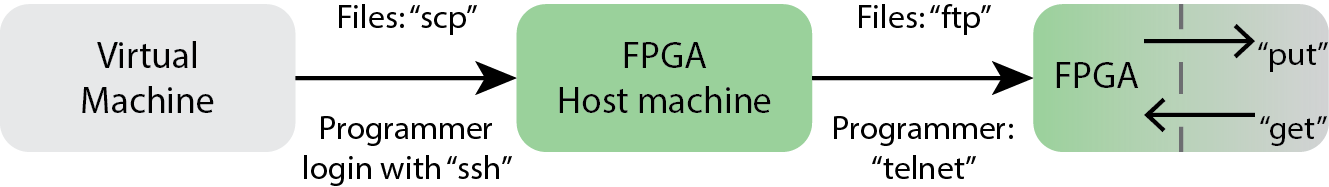
\includegraphics[width=300px]{Pictures/hoprecht}%
\caption{Ubuntu commands for putting files on and navigating to the FPGAs}%
\label{fig:hoppen}%
\end{figure}

For the first lab, the \mcode{pixel\_satd\_8x4} kernel has to be:
\begin{itemize}
	\item extracted into a separate file
	\item supplemented to a proper .c file which can be compiled and run using the $\rho$-VEX
	\item included in the \mcode{makefile} that creates a \mcode{bytecode} and \mcode{bytedata} file of the kernel
	\item debugged
\end{itemize}

Looking back, the debugging part has been chasing us all the way through the lab. Not only did we suffer from bugs in our source code, the $\rho$-VEX itself did also have shortcomings that had to be circumvented by downloading several fixes, competing for FPGA availability and break downs of the entire host machine due to unsufficient capacity for the amount of students.

